\documentclass[border=12pt]{standalone}
\usepackage{amsmath, amssymb}
\usepackage{tikz}
\definecolor{ring0}{HTML}{0033CC}
\definecolor{ring1}{HTML}{0066FF}
\definecolor{ring2}{HTML}{0099FF}
\definecolor{ring3}{HTML}{00CCCC}
\definecolor{ring4}{HTML}{00CC66}
\definecolor{ring5}{HTML}{33CC00}
\definecolor{ring6}{HTML}{99CC00}
\definecolor{ring7}{HTML}{CCCC00}
\definecolor{ring8}{HTML}{FF9900}
\definecolor{ring9}{HTML}{FF6600}
\definecolor{ring10}{HTML}{FF3300}
\definecolor{ring11}{HTML}{CC0000}
\definecolor{gap0}{HTML}{E53935}
\definecolor{gap1}{HTML}{1E88E5}
\definecolor{gapfar}{HTML}{CCCCCC}
\begin{document}
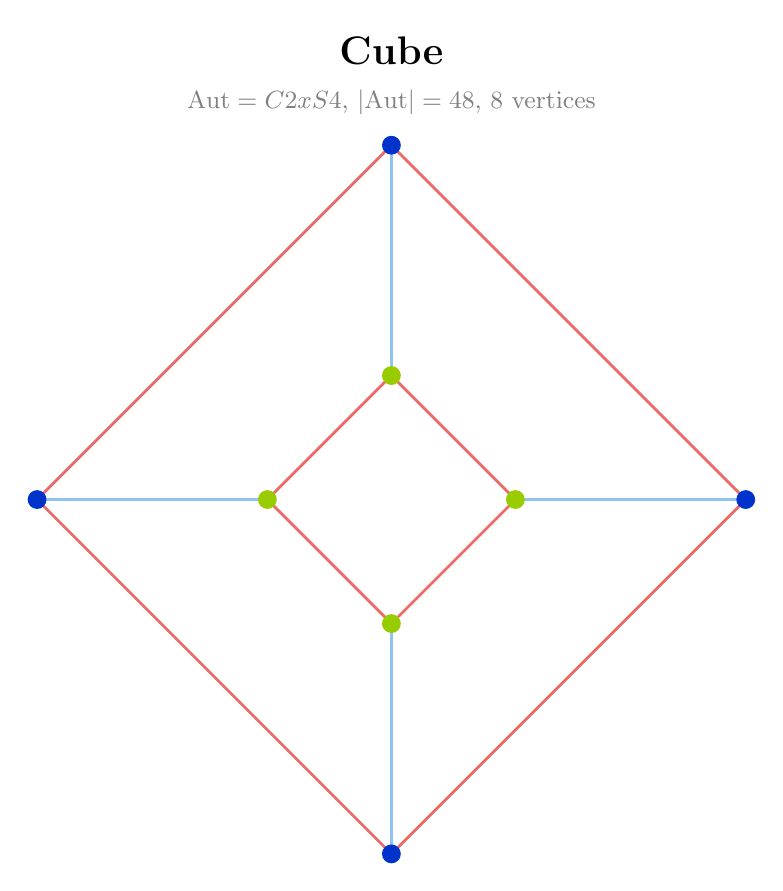
\begin{tikzpicture}
\node[font=\Large\bfseries] at (0, 5.70) {Cube};
\node[font=\small, text=gray] at (0, 5.05) {$\mathrm{Aut} = C2 x S4$, $|\mathrm{Aut}| = 48$, 8 vertices};
\draw[line width=0.80pt, gap1, opacity=0.50] (0.000, 4.500) -- (0.000, 1.575);
\draw[line width=0.80pt, gap1, opacity=0.50] (1.575, -0.000) -- (4.500, -0.000);
\draw[line width=0.80pt, gap1, opacity=0.50] (-4.500, 0.000) -- (-1.575, 0.000);
\draw[line width=0.80pt, gap1, opacity=0.50] (-0.000, -1.575) -- (-0.000, -4.500);
\draw[line width=1.00pt, gap0, opacity=0.75] (0.000, 4.500) -- (4.500, -0.000);
\draw[line width=1.00pt, gap0, opacity=0.75] (0.000, 4.500) -- (-4.500, 0.000);
\draw[line width=1.00pt, gap0, opacity=0.75] (0.000, 1.575) -- (1.575, -0.000);
\draw[line width=1.00pt, gap0, opacity=0.75] (0.000, 1.575) -- (-1.575, 0.000);
\draw[line width=1.00pt, gap0, opacity=0.75] (1.575, -0.000) -- (-0.000, -1.575);
\draw[line width=1.00pt, gap0, opacity=0.75] (4.500, -0.000) -- (-0.000, -4.500);
\draw[line width=1.00pt, gap0, opacity=0.75] (-4.500, 0.000) -- (-0.000, -4.500);
\draw[line width=1.00pt, gap0, opacity=0.75] (-1.575, 0.000) -- (-0.000, -1.575);
\fill[ring0] (0.000, 4.500) circle (3.4pt);
\fill[ring6] (0.000, 1.575) circle (3.4pt);
\fill[ring6] (1.575, -0.000) circle (3.4pt);
\fill[ring0] (4.500, -0.000) circle (3.4pt);
\fill[ring0] (-4.500, 0.000) circle (3.4pt);
\fill[ring6] (-1.575, 0.000) circle (3.4pt);
\fill[ring6] (-0.000, -1.575) circle (3.4pt);
\fill[ring0] (-0.000, -4.500) circle (3.4pt);
\end{tikzpicture}
\end{document}